\documentclass{article}[10]
\pdfpagewidth=8.5in
\pdfpageheight=11in

\usepackage{PACISE} % Include the custom commands from the PACISEPaper.sty

\usepackage{times} % Use the postscript times font
\usepackage{soul} % Strikeout, underline, space out, etc.
\usepackage{url}
\usepackage[hidelinks]{hyperref} % hrefs
\usepackage[utf8]{inputenc} % Encode in utf8
\usepackage[small]{caption}
\usepackage{mathtools}
\usepackage{array}
\usepackage{graphicx}
\usepackage{amsmath}
\usepackage{booktabs}
\usepackage{framed}
\usepackage{float}
\usepackage{relsize}
\usepackage[ruled]{algorithm2e}
\usepackage{lipsum}
\usepackage{tkz-graph}
\usepackage{titlesec}
\usetikzlibrary{arrows}

\urlstyle{same}

\title{A COMPARISON OF AUTOMATIC EXTRACTIVE TEXT SUMMARIZATION TECHNIQUES}

\author{
Alex Day$^1$
\and
Soo Kim$^1$
\affiliations
$^1$Clarion University of Pennsylvania, Computer Information Science Department\\
\emails
\href{mailto:A.D.Day@eagle.clarion.edu}{A.D.Day@eagle.clarion.edu},
\href{mailto:skim@clarion.edu}{skim@clarion.edu}
}


\begin{document}

\maketitle

\titleformat{\section}
  {\normalfont\fontsize{10}{0}\bfseries}{\thesection}{1em}{}

\setlength{\parskip}{0em}
\section*{ABSTRACT}
\setlength{\parskip}{1em}
    Text summarization is a method of shortening a document by producing a set
    of representative information. It can be generally categorized into
    extractive and abstractive summarization. Extractive summarization - the
    focus of this paper - is extracting sentences and phrases that are already
    present within the document in order to produce an outline. Term Frequency -
    Inverse Document Frequency is a score-based summarization technique that
    assigns a numerical value to each term in the document and then scores the
    relative importance of each sentence. TextRank is a graph-based
    summarization technique which uses a graph data structure to rank the
    document into the relevant sentences. This paper describes those two
    extractive text summarization methods and presents the results of running
    the algorithms on three different corpora: \textit{Moby-Dick} by Herman
    Melville, a selection of Reuters news articles, and a selection of posts on
    Reddit. The algorithms rank the sentences by relevance to the document, take
    the top five sentences, and return them as a summary.

\begin{keywords}
Natural Language Processing, Extractive Summarization, TF-IDF, TextRank, Graph Summarization, Ranked Summarization
\end{keywords}

\titleformat{\section}
  {\normalfont\fontsize{12}{10}\bfseries}{\thesection}{1em}{}


\section{Introduction}
% TODO
% Explain the basics of what we are trying to do
The goal of automatic summarization is finding a small amount of information that is most representative of a larger set of information. This can be done with images, video, or text.  The need for efficient and accurate summarization algorithms has only risen with the onset of the Internet. According to the study done by the Media Insight Project  \cite{rosenstiel2014personal}, about 6 in 10 Americans only read the headline of a news article and delve no deeper than that. If people are willing to read one sentence headline, they may also be willing to read a 5-sentence summary. This summary would result in the people getting more information about the story, letting them be better informed.

Automatic summarization is categorized broadly into two techniques: extractive and abstractive. Extractive summarization takes words and sentences already within the document to form a summary, whereas abstractive summarization tries to understand the information within the document and summarize it by creating new sentences.

Arguably, one of the most cited and earliest works in automatic summarization is that of Luhn \cite{luhn1958automatic}, which provides an overview of work by IBM in automatically generating technical paper abstracts using an early TF-IDF-esq algorithm. The original idea for this paper was inspired by Samir Bajaj \cite{bajajshakespeare} and his paper entitled \textit{Shakespeare in One Hundred Words}. Samir investigated four abstractive summarization methods, such as TF-IDF–based relevance ranking, K-means clustering algorithm, singular value decomposition, and PageRank. In addition, Dipanjan Das, et. al  \cite{das2007survey} surveyed different summarization methods: naive-Bayes methods, rich features and decision trees, hidden Markov models, log-linear models,  neural networks and third party features, deep natural language analysis methods, abstraction and information fusion, topic-driven summarization and maximal marginal relevance, graph spreading activation, centroid-based summarization, and so on. Dipanjan Das, et. al discussed some unconventional
approaches that can be useful in the future of summarization research and elaborated some evaluation techniques as well as the standards for evaluating summaries automatically.

This paper focuses on extractive summarization methods: Term Frequency - Inverse Document Frequency (TF-IDF) and TextRank. These algorithms summarize a document in completely different ways. TF-IDF scores each sentence on relevance to the document as a whole, while TextRank is a graph-based sorting algorithm that separates each sentence into a node and links it to other sentences based on similarity. The methods TF-IDF and TextRank are explained in Section 2 and Section 3, respectively. The implementation details and the results of running these algorithms on three different corpora are presented in Section 4 and Section 5. Finally, the conclusion is given in Section 6.

\section{Term Frequency - Inverse Document Frequency}
Term Frequency-Inverse Document Frequency (TF-IDF) \cite{Beel2016-11Resea-32348} is one of the most used weighting schemes for term importance. TF-IDF assigns a value to each word in a document and this assigned score indicates the importance of the word to the document. It is proportional to the frequency of the term in the document and offset by the term's use throughout the whole corpus. This offset ensures that common words such as "the", "and", "or", etc., do not skew the score since they have such low inverse document frequencies. The calculations used are shown in Equation \ref{raw-tfidf}. It should be noted that Equation \ref{raw-tfidf} is one of the ways to calculate a TF-IDF score \cite{bajajshakespeare} and other non-logarithmic scales can be used, depending on the desired outcome.

\begin{equation}
\label{raw-tfidf}
    \begin{aligned}
        tf(t, d) &= f_{t, d}\\
        idf(t, D) &= log\frac{\abs{D}}{\abs{\{d \in D : t \in d\}}}\\
        tfidf(t, d, D) &= tf(t, d) \times idf(t, D)
    \end{aligned}
\end{equation}
\begin{conditions}
    t     &  Term to calculate the score of \\
    d     &  Document to calculate the score relative of \\
    D     &  Corpus of documents such that $d \in D$
\end{conditions}


The  \textit{tfidf} is a score that is assigned only to a specific word within a document, so it cannot be used directly to assign importance-values to a whole sentence. In order to get an importance-value of a whole sentence, the average of each \textit{tfidf} score is taken for every word within that sentence as shown in Equation \ref{avg-tfidf}.

\begin{equation}
	\label{avg-tfidf}
	\begin{aligned}
		\mathlarger{\frac{1}{\abs{S}}\times\sum\limits_{w \in S} tfidf(w, d, D) }
	\end{aligned}
\end{equation}
\begin{conditions}
    w     &  Word present in $d$ to calculate the score of \\
    S     &  Set of sentences in $d$ \\
    d     &  Document to calculate the scores relative of \\
    D     &  Corpus of documents such that d $\in$ D
\end{conditions}


Algorithm \ref{algo-tfidf} uses both of these equations. It calculates the \textit{tfidf} score for each sentence in a document and then returns a list of the sentences within the document sorted by the sentence scoring. The term frequency score for each term is individual for the document that the term is in. The inverse document frequency of a term will only have to be recalculated each time when a document is added to the corpus. The order of the sentences as they appear in the original document is also important to the summary. In order to represent this fact, the sentences in the summary are sorted by the original location of the sentences within the document.

\begin{algorithm}[ht]
    \hspace*{6px} \textbf{Input}: A set of documents, $C$ \\
    \hspace*{6px} $\:\:\:\:\:\:\:\:\:\:\:\:$ A document to summarize, $D$, such that $D\in C$ \\
    \hspace*{6px} \textbf{Output}: A list of sentences sorted based on relevance


    tfidf\_scores[] $\leftarrow$ 0\;
    \For{sentence $\in\:D$}
    {
        tfidf\_sum $\leftarrow$ 0\;

        \For {word $\in$ sentence}
        {
            tfidf\_sum += $tfidf$(word, document, corpus)\;
        }

        tfidf\_scores[word] $\mathlarger{\leftarrow\:\frac {tfidf\_sum}{ \abs{D} }}$\;
    }
    return \textbf{sorted}(tfidf\_scores)
    \caption{Return the ranked sentences for a document using TF-IDF}\label{algo-tfidf}
\end{algorithm}

\section{TextRank}
PageRank is a web page ranking algorithm developed for use with the Google search engine \cite{page1999pagerank}. PageRank determines the importance of each web page returned in the search results through the number of web pages that link back to it. For example, a page such as an article on Wikipedia is important because many pages are linked to it. TextRank \cite{mihalcea2004textrank} takes the same graph-oriented approach as PageRank; however it deems a node in the graph important if that node is similar to many other nodes.

TextRank begins by separating each of the sentences in documents into nodes in a graph. Each node is linked to every other node with the weight of that edge being the similarity score. The most relevant sentences are represented by the nodes with the highest cumulative total of all edges that are connected to the node. The algorithm used in the code for this paper is shown in Algorithm \ref{algo-tr} and an example of a document similarity graph is shown in Figure \ref{graph-tr}. In this example, the document consists of three sentences $S_1$, $S_2$, and $S_3$. $S_1$ has the similarity score 0.3 with $S_2$ and the similarity score 0.9 with $S_3$, so the sum of the similarity scores for $S_1$ is 1.2. The three sentences would be ranked in  $[S_{1}, S_{3}, S_{2}]$ with their sums of similarity scores of all connected edges being $[1.2, 1.0, 0.4]$, respectively. As the result, $S_1$ would be ranked as the most relevant sentence and selected for the summary.

\begin{figure}[ht]
\renewcommand{\figurename}{Figure}%
\centering
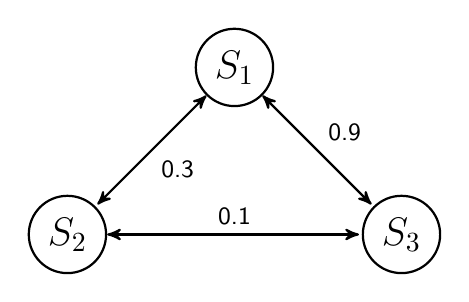
\begin{tikzpicture}[<->,>=stealth',shorten >=1pt,auto,node distance=3cm,
                    thick,main node/.style={circle,draw,font=\sffamily\Large\bfseries}]

  \node[main node] (1) {$S_1$};
  \node[main node] (2) [below left of=1] {$S_2$};
  \node[main node] (3) [below right of=1] {$S_3$};

  \path[every node/.style={font=\sffamily\small}]
    (1) edge node {0.9} (3)
        edge node {0.3} (2)
    (2) edge node {0.1} (3);
\end{tikzpicture}

\caption{A sentence similarity graph for a document containing the sentences $S_{1},\;S_{2},\;$ and $S_{3}$ represented as nodes on the graph where the edges represent the sentence similarities}
\label{graph-tr}
\end{figure}


\begin{algorithm}[ht]
    \hspace*{6px} \textbf{Input}: A set of documents, $C$ \\
    \hspace*{6px} $\:\:\:\:\:\:\:\:\:\:\:\:$ A document to summarize, $D$, such that $D\in C$ \\
    \hspace*{6px} \textbf{Output}: A list of sentences sorted based on relevance

    G $\leftarrow$ empty graph \;
    \For{sentence $\in\:D$}
    {
        G.add\_node(sentence)\;
    }

    \For{outer node $\in$ G}
    {
        \For{inner node $\in$ G : inner node $!=$ outer node}
        {
            G.add\_vertex(outer\_node, inner\_node, similarity(inner\_node, outer\_node))\;
        }
    }

    sentence\_scores[] $\leftarrow$ 0\;
    \For{node $\in$ G}
    {
        sentence\_scores[node] = sum(G.get\_edges(node))\;
    }

    return \textbf{sorted}(sentence\_scores)
    \caption{Return the ranked sentences for a document using TextRank}\label{algo-tr}
\end{algorithm}

TextRank relies on a concept called sentence embeddings to calculate the sentence similarity. A sentence embedding is a vector representation of that sentence. This vector representation is usually produced by a neural network that has been trained on a corpus. The neural network maps the sentence to a vector representation. It can glean this information from position in the document or surrounding sentences.

Cosine similarity is used to calculate the similarity of two vectors rather than Euclidean distance due to the high dimensionality of the data. Cosine similarity measures the cosine of the angle between two vectors, whereas the Euclidean distance calculates the length of the line segment that connects them. For example, two similar vectors, $the\:man\:is\:good$ and $the\:king\:is\:just$, could be far apart from each other in distance, but this may only due to the different context they are used in. However, the result of the cosine similarity is the angle between the two vectors, so it will take into account more the similarity of specific indices of each vector.

It may be simpler to think first about word embeddings. The same technique can be used to produce vectors for words. Translating words to vectors opens up the possibility of performing vector operations on words. For example, one can produce the vectors for king, queen, woman, and man. Then the vector resulting from the operation $king - (man + woman)$ would be relatively close to $queen$. As well as simple addition and subtraction, the same similarity calculations for sentence embeddings can be performed in word embeddings.

\section{Implementation}
All of the programs were written in Python 3.6, using the following packages: NetworkX \cite{networkX}, PRAW \cite{PRAW}, NLTK \cite{hermann2015teaching}, and NumPy \cite{numpy}. The codes can be found at the authors' GitHub repository \cite{DayAutomaticAnon}.

\section{Results}
These two algorithms have been tested on three separate corpora composed in three different styles. The first is the novel \textit{Moby-Dick} by Herman Melville, which is a semi-formal fictional novel. The second is a corpus of Reuters news articles. The third, and last corpus, is informal posts on the Reddit subreddit, ``Legal Advice." The main purpose of testing the algorithms on three separate corpora was to determine how each algorithm will act in different use cases. Section 5.1 presents the summary results of \textit{Moby-Dick}, Section 5.2 presents the summary results of Reuters news articles, and Section 5.3 presents the summary results of Legal Advice subreddit. Note that each summary contains five sentences as a result.

\subsection{Moby-Dick}
The complete work of \textit{Moby-Dick} was obtained through the NLTK package \cite{bird2009natural}. This novel was then split into chapters and each chapter was summarized. The corpus that was used contained all 135 chapters and approximately 253,129 words. Figure 2 shows the summary result of Chapter 1 of \textit{Moby-Dick} using TF-IDF, and Figure 3 shows the summary result of Chapter 1 of \textit{Moby-Dick} using TextRank.

\begin{figure}
    \begin{framed}
        - On the contrary, passengers themselves must pay.\\
        - Whaling voyage by one ishmael."\\
        - For to go as a passenger you must needs have a purse, and a purse is but a rag unless you have something in it.\\
        - Why upon your first voyage as a passenger, did you yourself feel such a mystical vibration, when first told that you and your ship were now out of sight of land?\\
        - Right and left, the streets take you waterward.\\
        \caption{Summary of Chapter 1 of \textit{Moby-Dick} using TF-IDF}
        \label{results-tfidf-moby}
    \end{framed}
\end{figure}

\begin{figure}
    \begin{framed}
        - Deep into distant woodlands winds a mazy way, reaching to overlapping spurs of mountains bathed in their hill-side blue.\\
        - Why did the poor poet of tennessee, upon suddenly receiving two handfuls of silver, deliberate whether to buy him a coat, which he sadly needed, or invest his money in a pedestrian trip to rockaway beach?\\
        - Well, then, however the old sea-captains may order me about -- however they may thump and punch me about, I have the satisfaction of knowing that it is all right; that everybody else is one way or other served in much the same way -- either in a physical or metaphysical point of view, that is; and so the universal thump is passed round, and all hands should rub each other's shoulder-blades, and be content.\\
        - But wherefore it was that after having repeatedly smelt the sea as a merchant sailor, I should now take it into my head to go on a whaling voyage; this the invisible police officer of the fates, who has the constant surveillance of me, and secretly dogs me, and influences me in some unaccountable way -- he can better answer than any one else \\
        - With other men, perhaps, such things would not have been inducements; but as for me, I am tormented with an everlasting itch for things remote.\\
        \caption{Summary of Chapter 1 of \textit{Moby-Dick} using TextRank}
        \label{results-textrank-moby}
    \end{framed}
\end{figure}

\subsection{Reuters News Articles}
The second round of testing was done on another corpus from NLTK \cite{bird2009natural}. The corpus contains 10,000 news articles from Reuters. These articles combine works from different writers which produce interesting results. However, they are all achieving the same tone and follow Reuters style guide. Figure 4 shows the summary result of Reuters news articles using TF-IDF, and Figure 5 shows the summary result of Reuters news articles using TextRank.

\begin{figure}
    \begin{framed}
        - New crop sales were also light and all to open ports with  June/July going at 1,850 and 1,880 dlrs and at 35 and 45 dlrs  under New York july, Aug/Sept at 1,870, 1,875 and 1,880 dlrs  per tonne FOB.\\
        - March/April sold at  4,340, 4,345 and 4,350 dlrs.\\
        - April/May butter went at 2.27 times New York May, June/July  at 4,400 and 4,415 dlrs, Aug/Sept at 4,351 to 4,450 dlrs and at  2.27 and 2.28 times New York Sept and Oct/Dec at 4,480 dlrs and  2.27 times New York Dec, Comissaria Smith said.\\
        - Cake sales were registered at 785 to 995 dlrs for  March/April, 785 dlrs for May, 753 dlrs for Aug and 0.39 times  New York Dec for Oct/Dec.\\
        - Liquor sales were limited with March/April selling at 2,325  and 2,380 dlrs, June/July at 2,375 dlrs and at 1.25 times New  York July, Aug/Sept at 2,400 dlrs and at 1.25 times New York  Sept and Oct/Dec at 1.25 times New York Dec, Comissaria Smith  said.
        \caption{Summary of a news article using TF-IDF}
        \label{results-tfidf-cnn}
    \end{framed}
\end{figure}
\begin{figure}
    \begin{framed}
        - There are doubts as to how much of this cocoa would be fit  for export as shippers are now experiencing difficulties in  obtaining +Bahia superior+ certificates.\\
        - March/April sold at  4,340, 4,345 and 4,350 dlrs.\\
        - April/May butter went at 2.27 times New York May, June/July  at 4,400 and 4,415 dlrs, Aug/Sept at 4,351 to 4,450 dlrs and at  2.27 and 2.28 times New York Sept and Oct/Dec at 4,480 dlrs and  2.27 times New York Dec, Comissaria Smith said.\\
        - Cake sales were registered at 785 to 995 dlrs for  March/April, 785 dlrs for May, 753 dlrs for Aug and 0.39 times  New York Dec for Oct/Dec.\\
        - Liquor sales were limited with March/April selling at 2,325  and 2,380 dlrs, June/July at 2,375 dlrs and at 1.25 times New  York July, Aug/Sept at 2,400 dlrs and at 1.25 times New York  Sept and Oct/Dec at 1.25 times New York Dec, Comissaria Smith  said.

        \caption{Summary of a news article using TextRank}
        \label{results-textrank-cnn}
    \end{framed}
\end{figure}

\subsection{Legal Advice Subreddit}
The last corpus is a collection of posts from a site called Reddit. Reddit is a website that allows the general public to post within forums dedicated to specific topics. The forum chosen for this corpus is called ``Legal Advice". This forum contains posts by users describing situations for which they believe they need advice from legal counsel. Using the Python package PRAW \cite{PRAW}, the top 1,000 most liked posts of the last 30 days were retrieved, and then the posts long enough to warrant a summary were passed through the algorithms. Figure 6 shows the summary result of Reddit legal advice posts using TF-IDF, and Figure 7 shows the summary result of Reddit legal advice posts using TextRank.

\begin{figure}
    \begin{framed}
        - I will just be saying MY home or MY driveway so I don't have to keep typing "my parent's driveway" or "my parent's home" over and over.\\
        - My parent's neighbor's kid (a very immature 20 year old) has a beater he leaves parked in front of my parent's front yard.\\
        - Now the parents are retaliating too.They finally moved the beater, but only to move their cars from the driveway to taking up the two spaces in front of our yard adjacent to their driveway.\\
        - The one car parked just enough to have the front poking into our driveway.\\
        - TLDR - neighbors parked all their cars in front of my parents home and wont move them, only rearrange them.\\
        \caption{Summary of a Reddit posts using TF-IDF}
        \label{results-tfidf-reddit}
    \end{framed}
\end{figure}

\begin{figure}
    \begin{framed}
        - These neighbors moved in a year or two ago and have made life so uncomfortable for my parents they are actually talking about selling their home to move, their marriage home with ALL the memories.\\
        - He has it parked in the middle so that it takes up ALL the space and no one can park on either side of it without blocking a driveway.\\
        - I assumed mom would just tell 'Billy, go move your damn car' or something and it would be taken care of.\\
        - I get the dad yelling at me to *** off and get off his property as the mom (from another room) starts bellowing about how I did NOT just tell her how to parent and he can do whatever he wants and **** me and my parents.\\
        - Not only do they say the street parking is technically public parking and they can't officially complain about it, but they complain the neighbors will only retaliate worse.\\
        \caption{Summary of a Reddit posts using TextRank}
        \label{results-textrank-reddit}
    \end{framed}
\end{figure}

\flushbottom

\section{Conclusion}
Both TF-IDF and TextRank algorithms produced a much more representative summary of the Reddit posts, while they performed decently with the fictional works and the formally styled news articles. This disparity between summary quality may be because the Reddit posts are focused only around one situation that happened, whereas in both \textit{Moby-Dick} and the news articles, the reader is presented with a background story and sometimes a story arc. The algorithms presented for extractive summarization do not perform optimally when presented with a story line. However, if a summary needs to be generated for a news article focused on one specific topic or a short story focused on one situation, both TF-IDF and TextRank are good choices.

It seems that TextRank has a tendency to favor longer sentences. This could be because longer sentences have more space to include any buzzwords. It can be offset by scaling the similarity score for each sentence by the length, just like the TF-IDF algorithm, although this behavior may be preferred for a more complex corpus.

In the future, abstractive summarization will be explored to determine an algorithm that returns a summary by utilizing natural grammar structures. This will be done with the aim of producing more representative summaries, specifically for \textit{Moby-Dick} and the Reuters articles. And, the usefulness of neural networks, specifically long short-term memory neural networks (recurrent neural network) \cite{yao2014spoken}, will be tested to increase the performance. In addition, evaluation methods of text summarization will be investigated to measure the quality of the summaries.

\makeatletter
\renewenvironment{thebibliography}[1]
     {\section*{\refname}%
      \@mkboth{\MakeUppercase\refname}{\MakeUppercase\refname}%
      \list{\@biblabel{\@arabic\c@enumiv}}%
           {\settowidth\labelwidth{\@biblabel{#1}}%
            \setlength{\itemindent}{\dimexpr\labelwidth+\labelsep}
            \leftmargin\z@
            \@openbib@code
            \usecounter{enumiv}%
            \let\p@enumiv\@empty
            \renewcommand\theenumiv{\@arabic\c@enumiv}}%
      \sloppy
      \clubpenalty4000
      \@clubpenalty \clubpenalty
      \widowpenalty4000%
      \sfcode`\.\@m}
     {\def\@noitemerr
       {\@latex@warning{Empty `thebibliography' environment}}%
      \endlist}
\makeatother
\bibliographystyle{PACISE}
\bibliography{biblio}

\end{document}
